\section{Descrizione del Modello}
Il modello considerato \cite{mostafizi2019agent} é un sistema multi-agente che prevede l'evacuazione della città di Seaside, Oregon in caso di tsunami di auto e pedoni.
%
% TODO: riscrivere
L'evacuazione non include le conseguenze del terremoto che avviene prima dello tsunami e viene considerata iniziare alla fine di questo.
Il modello è basato sull'uso di dati GIS per la distribuzione della popolazione, la rete stradale ed i rifugi.

%
Per la distribuzione della popolazione é stato considerato uno scenario a mezzogiorno di un fine settimana di estate,
che presenta una maggiore concentrazione di residenti sulla spiaggia e nel centro della città
La popolazione sulla costa e nel centro é distribuita normalmente,
mentre quella nella zona residenziale é distribuita uniformemente (Fig. \ref{fig:population}).

\begin{figure}[ht]
  \centering
  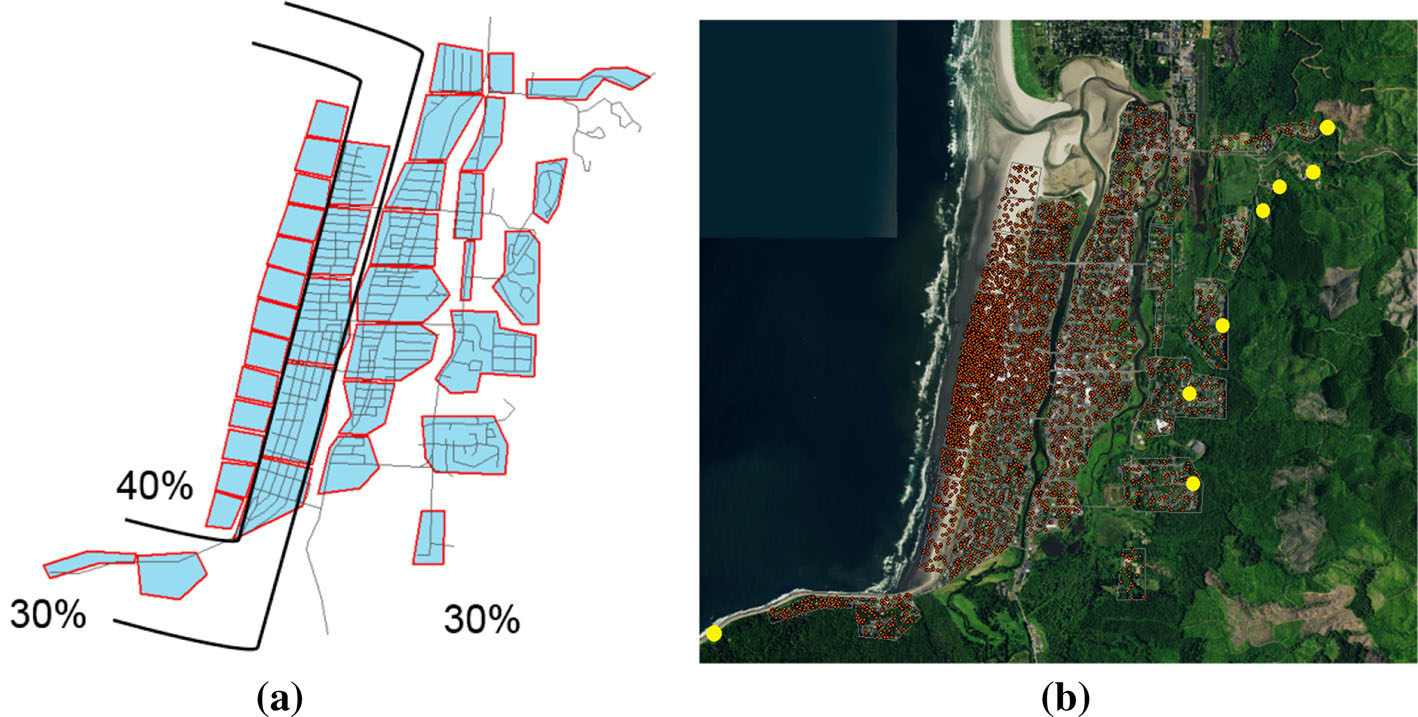
\includegraphics[width=0.82\textwidth]{images/population}
  \caption{Distribuzione della popolazione nello scenario considerato.
    (a) Mostra le aree in cui è distribuita la popolazione, divise nelle tre macro aree: costa, centro, zona residenziale.
    (b) Immagine satellitare con la distribuzione della popolazione.}
  \label{fig:population}
\end{figure}

\subsection{Ambiente}
L'ambiente é composto dalla rete stradale della città con i relativi rifugi e dello tsunami.

% TODO: riscrivere
La rete stradale é rappresentata da un grafo, i cui nodi corrispondono alle intersezioni e gli archi alle strade.
Tutte le strade sono considerate a senso unico, con una sola corsia e con una velocità limite di 55 km/h.

8 delle intersezioni sono marcate come rifugi con capacità illimitata.

Lo tsunami é rappresentato da una griglia discreta, dove ogni cella contiene i valori temporali di altezza delle onde.
I dati usati in questo progetto sono quelli calcolati dal modello di inondazione ComMIT/MOST \cite{titov1997implementation} per la zona di subduzione della Cascadia.


\subsection{Agenti}
La simulazione può prevedere diversi tipi di agenti: residenti, pedoni e auto.

\subsubsection{Residenti}
All'inizio dell'evacuazione i residenti si trovano all'esterno di edifici e auto
e autonomamente scelgono come evacuare. % TODO: mmmmh
Un residente può scegliere diverse modalità per evacuare: a piedi o in auto e raggiungere un rifugio verticale oppure orizzontale.
Una volta che ogni agente decide in che modo evacuare non cambierà scelta per tutta la simulazione.

\vspace*{4mm}
Il tempo impiegato per prepararsi all'evacuazione (milling time) é modellato tramite
la distribuzione di Rayleigh (Eq. \ref{eq:rayleigh}), con un tempo minimo ($\tau$) di 10 minuti
e un parametro di scala ($\sigma$) di 1.65.
Questo tempo comprende anche il raggiungimento del veicolo.

\begin{equation}
  f(x; \tau, \sigma) = \frac{(x - \tau)^2}{\sigma^2}e^{-{(x - \tau)^2}/(2\sigma^2)}
  \label{eq:rayleigh}
\end{equation}

Scaduto il tempo di preparazione l'agente si muove verso l'intersezione più vicina e
in base alla modalità scelta viene considerato un agente di tipo pedone o auto.
L'agente quindi inizia a seguire il percorso più breve per il rifugio più vicino raggiungibile, trovato tramite l'algoritmo A*.

Gli agenti durante l'evacuazione possono continuare sulla strada attuale o cambiare strada seguendo il percorso,
morire se l'altezza dell'onda nel punto in cui si trova é superiore o uguale a un parametro $H_c$,

\subsubsection{Pedoni}
La velocità di camminata viene stabilita tramite una distribuzione normale
con media 1.21 m/s e deviazione standard 0.20 m/s.
La velocità di ogni pedone rimane costante durante tutta l'evacuazione.

% Non viene gestita alcuna interazione Pedone-Pedone o Pedone-Auto.

\newpage
\subsubsection{Auto}
Ogni auto conteniene una sola persona per considerare il caso peggiore.
Le auto possono raggiungere la velocità massima imposta dalla strada, ovvero 55 km/h.

Il comportamento delle auto é modellato tramite il modello car-following, General-Motors.

La teoria sui modelli Car following descrivono come un veicolo ne segue un'altro
e cambi il proprio comportamenteo reagendo a quest'ultimo.

\begin{figure}[ht]
  \centering
  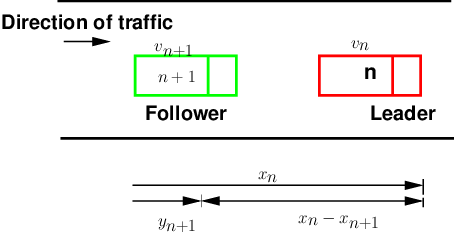
\includegraphics[width=0.9\textwidth]{images/GM.png}
  \label{fig:general-motors-img}
  \caption{schema generale dei modelli car following, dove n+1 è il veicolo corrente ed n quello di fronte, $v_{n+1}, v_{n}$ sono le rispetive velocità, mentre $x_{n+1}, x_{n}$ sono le rispettive posizioni è $x_{n} - x_{n + 1}$ è la distanza tra i due veicoli.}
\end{figure}

Secondo il modello General-Motors ogni auto risponde alle condizioni del traffico circostante esclusivamente accellerando o decelerando, l'accellerazione dipende dalla velocità del veicolo corrente, la sua posizione relativa e la velocità con il veicolo di fronte.
Basato sul concetto follow-the leader fondato su due assunzioni principali:
più veloce è il veicolo di fronte maggiore sarà la distanza tra i due veicoli,
inoltre una certa distanza di sicurezza dall'auto in fronte deve essere mantenuta.

\begin{equation}
  a_{n+1}^{t} = [ \frac{\alpha_{l, m} * (v_{n + 1}^{t})^{m} }{ (x_{n}^{t} - x_{n + 1}^{t})^{l}}][v_{n}^{t} - v_{n + 1}^{t}]
  \label{eq:general-motors-eq}
\end{equation}

\noindent
Equation 2: qui viene riportata l'equazione principale del modello General-Motors, 
dove l è un esponente di distanza con il veicolo di fronte che può assumere valori da +4 a -1,
m è un esponente di velocità con valori tra -2 a +2, $\alpha$ è un coefficiente di sensitività.






\section{Estensione del Modello}
In questa sezione verrano descritte le modifiche e le aggiunte effettuate da noi al modello base,
ma prima verrano evidenziate le limitazioni e mancanze del modello anche rispetto allo stato dell'arte.

La prima limitazione che si può notare del modello base è la gestione delle interazioni tra i vari agenti,
sia prima della partenza che durante l'evacuazione,
tale modello infatti considera esclusivamente le interazzioni auto-auto tramite il modello Car Following General Motor's,
ma non prevede nessuna interazione pedone-pedone o pedone-auto.
Nella letteratura sono molti i lavori anche network-based,
che considerano una velocità che cambia in base alla congestione sulla strada mentre il nostro modello considera pedoni con una velocità costante per tutta l'evacuazione.
Inoltre come anche visto nella letteratura nessun tipo di interazione viene gestita alle intersezioni cosa abbastanza irrealistica.
Un'ulteriore limitazione è la scelta dei percorsi sebbene la maggior parte dei lavori in letteratura utilizzino l'algoritmo di A*star, esistono altri metodi esempio Nash Equilibrium.
La rete stradale viene considerata con strade tutte one-way cosa non problematica se tutti gli agenti seguono sempre 
il percorso più breve per il rifugio più vicino a loro, ma che per altri algoritmi di routing potrebbe essere limitante.
Infine nessun tipo di considerazione viene effettivamente applicata sul comportamento dei turisti durante l'evacuazione,
che come visto in vari lavori risultà avere un peso notevole specialmente in periodi con tanti visitatori.

Come è stato appena descritto abbiamo visto come le interazioni tra gli agenti
abbiano ampio margine per essere rappresentate, in particolare ci si concentrerà sulle interazioni alle intersezioni
introducendo meccanismi di cooperazione tra i vari tipi di agente, ed aggiustando la velocità dei pedoni in base alla congestione
in modo da poter rappresentare uno scenario più realistico.


\subsection*{Modifiche alla rete stradale}
Prima di descrivere le varie aggiunte in questa sezione verrannò elencate le varie modifiche che sono state effettuate alla rete stradale.
Tutte le strade della rete sono state considerate come strade locali, ai link della rete è stata aggiunta la larghezza della strada,
inoltre la strada viene considerata a two-way per le auto ed sono presenti dei marciapiedi che sono bidirezionali.
In accordo con il Transportation System Plan del 2011 della città di Seaside, le stradi locali sono composte da due corsie per le auto
con una larghezza 34-40' di per una singola corsia, per tale lavoro la larghezza minima di 34' è stata considerato.
Inoltre due marciapiedi sono presenti per ambi i lati della strada con una larghezza 5' per ogniuno di essi.


\subsection{Speed Variability dei Pedoni}
I pedoni se non è presente alcuna auto nell'evacuazione allora percorrono il tragitto in strada, altrimenti procedono esclusivamente sui marciapiedi.

Una variabilità nella velocità di camminata è stata introdotta per i pedoni utilizzando il modello di weidman con una free-flow-speed di 1.34 m/s,
ed una jam-density di 5.4 p/m², il calcolo della densità è stato effettuato mediante la density ahead con una search length di 3m, come anche nei seguenti lavori GOTO, Tizio 2021.

Spiegare modello di weidmann.

\newpage

\subsection{Gestione degli Intersezioni}
Per la gestione delle intersezioni esclusivamente gli incroci a 4 strade sono stati considerati è trattati come intersezioni di tipo AWSC(All Way Stop Controlled) o TWSC(Two Way Stop controlled).
Tramite l'utilizzo di OpenStreetMap e GoogleMaps, sono state estratte manualmente le informazioni circa la posizione e nel case dei TWSC la direzione
di precedenza di tali tipi di incroci per la citta di Seaside, ottenendo la seguente immagine \ref{fig:intersections_map}.

Inoltre viene introdotta la gestione di zone di attraversamento agli incroci sia per le auto che per i pedoni.
La zona di attraversamento inizia e finisce ad una certa distanza su entrambi i lati dell'incrocio (la metà della larghezza dell'incrocio).

Sempre facendo riferimento al TSP del 2011 una larghezza dell'incrocio è stata definità come segue:
\begin{equation}
  \text{larghezza incrocio} = 2 * (\text{larghezza marciapiede} + \text{larghezza corsia stradale})
\end{equation}

Per i pedoni gli attraversamenti sono registrati in un dizionario indicizzato per direzione nell'intersezione dell'incrocio.
le direzioni considerate sono (LEFT, RIGTH, ORIGIN e STRAIGHT) ORIGIN è la direzione di provenienza.

Inoltre per i TWSC nelle intersezioni la presenza degli stop viene segnata, mediante una lista con il numero dell'intersezioni interessate.

\begin{figure}
  \begin{subfigure}[b]{0.9\textwidth}
    \centering
    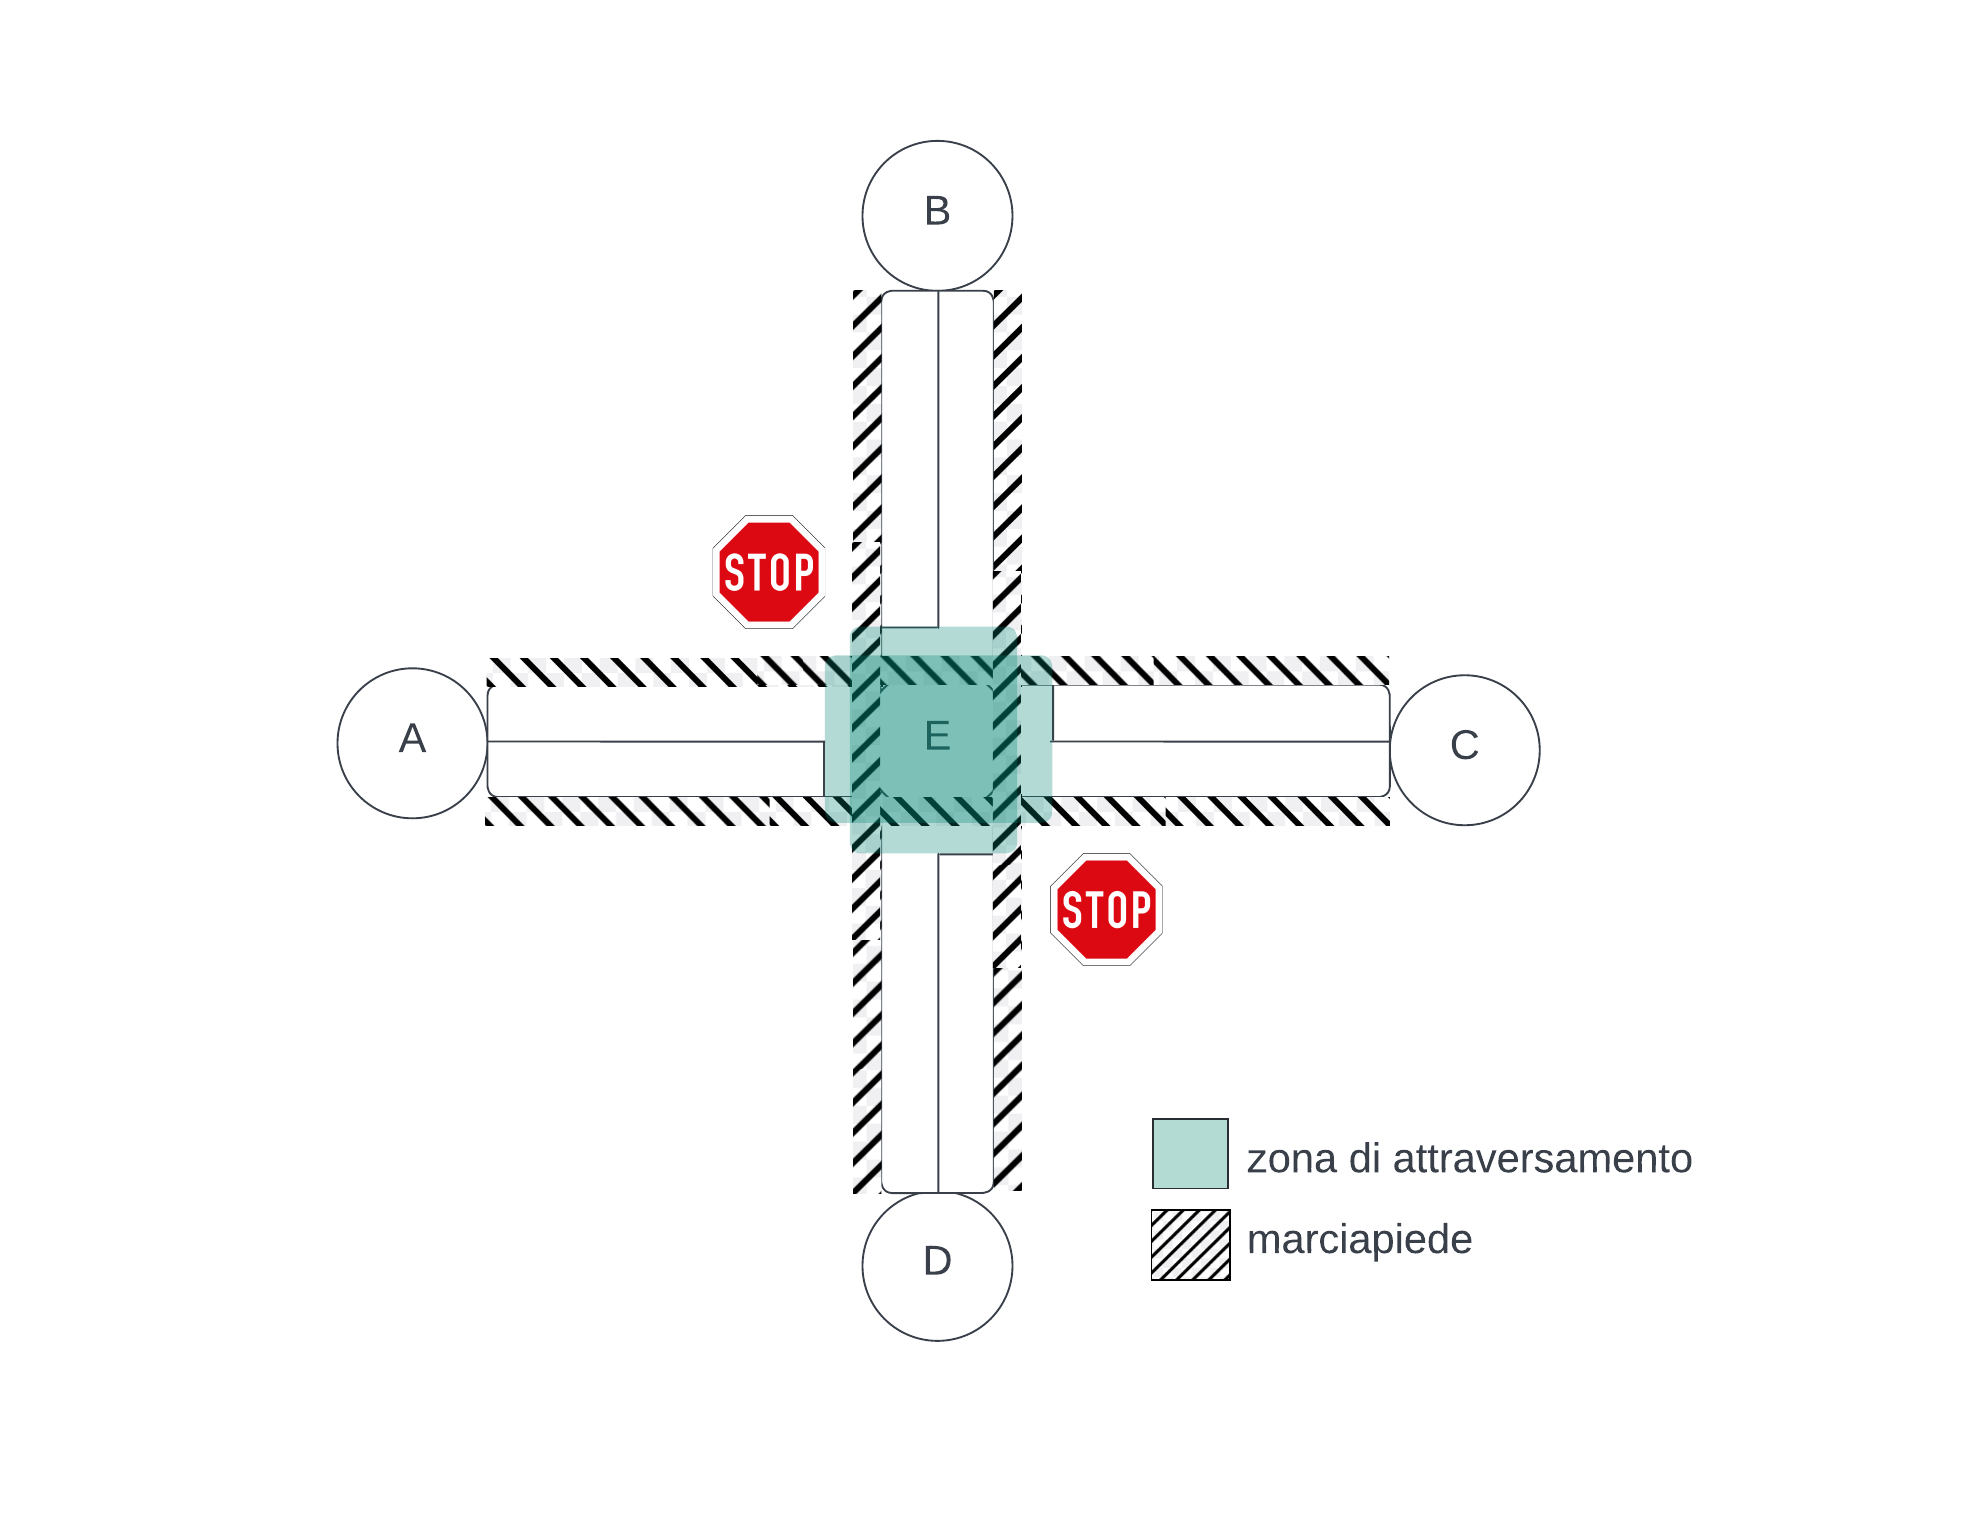
\includegraphics[width=\textwidth]{images/intersection state.png}
    \label{fig:intersection state}
    \caption{esempio di incrocio TWSC con zona di crossing evidenziata.}
  \end{subfigure}
  \hfill
  \centering
  \begin{subfigure}[b]{0.9\textwidth}
    \centering
    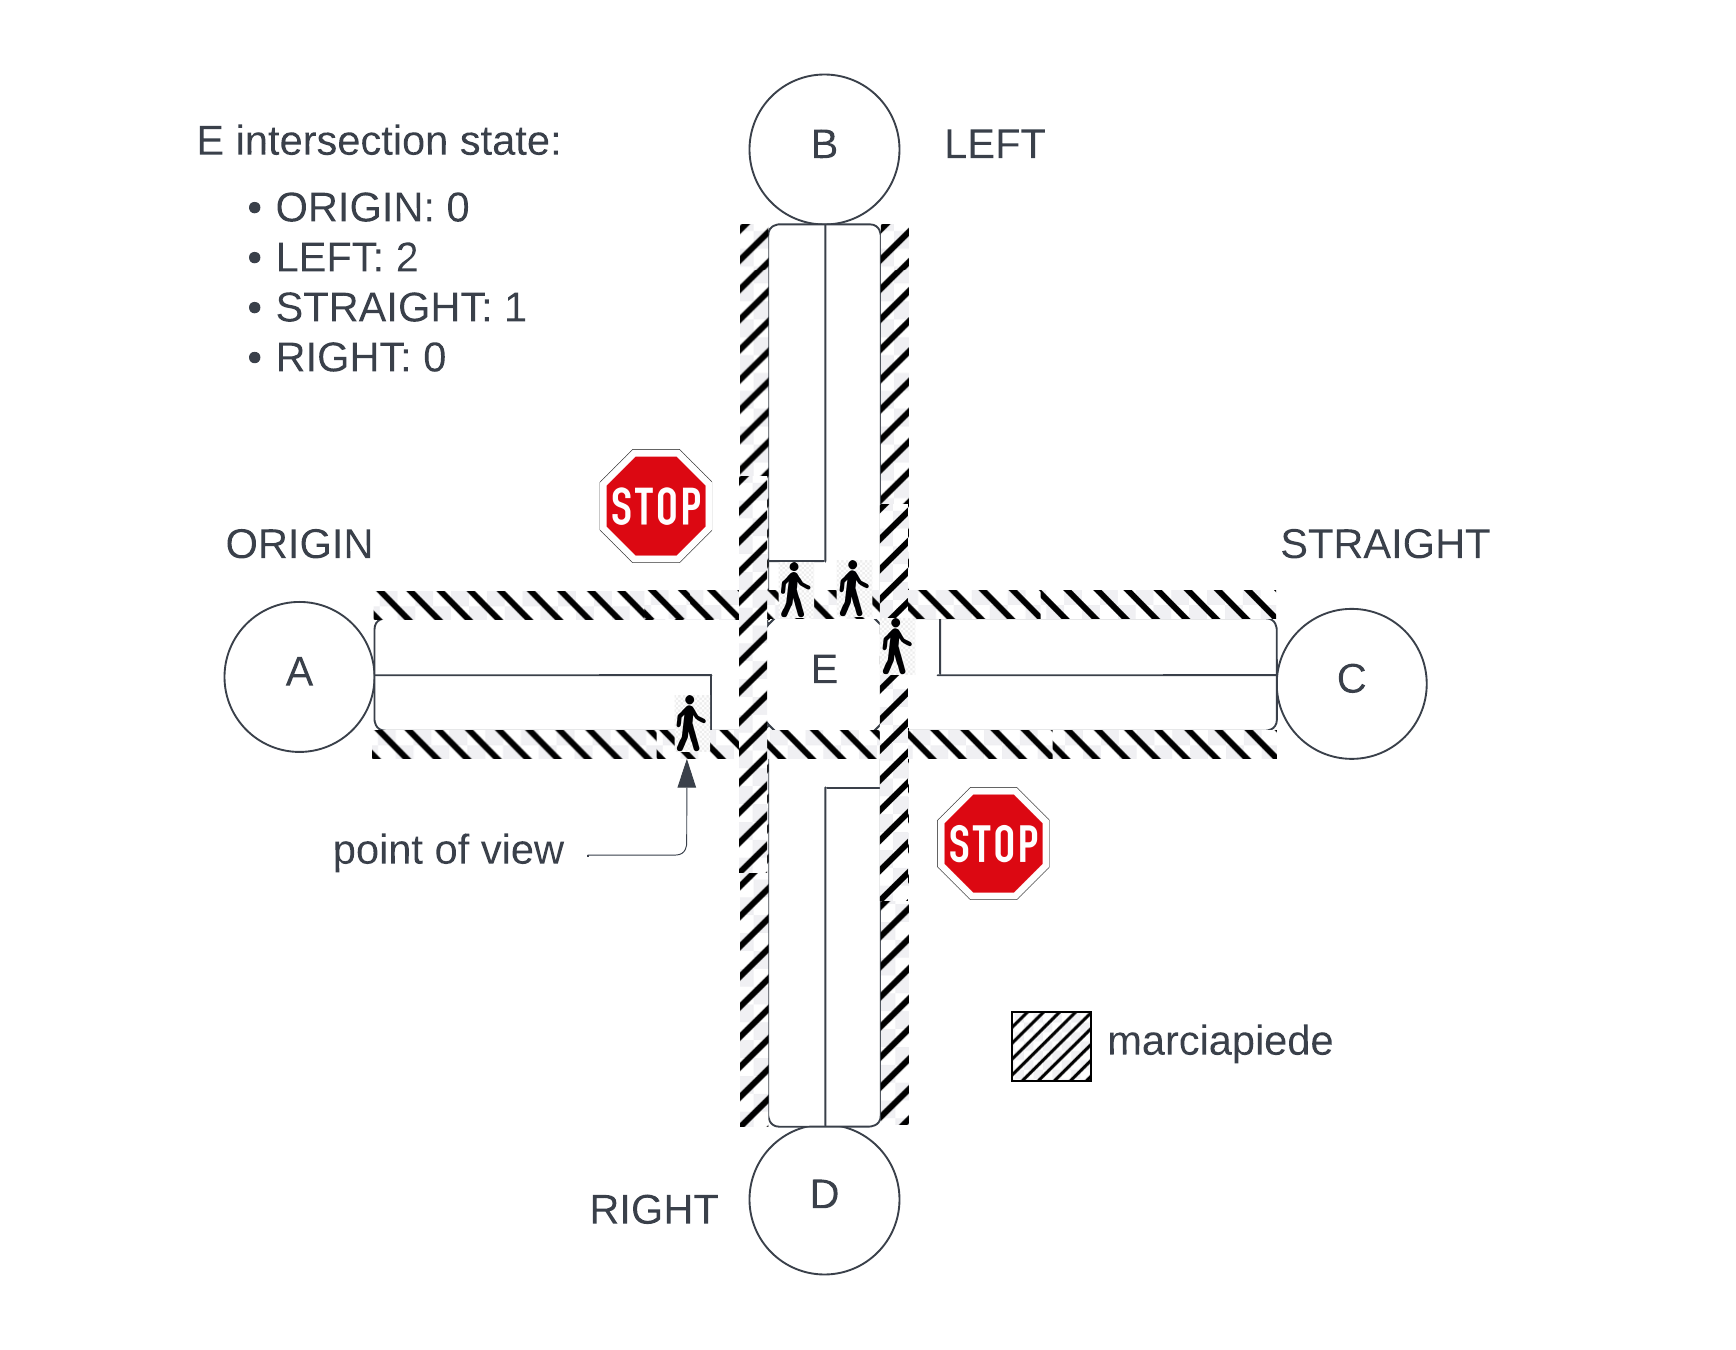
\includegraphics[width=\textwidth]{images/crosswalks.png}
    \label{fig:intersection state}
    \caption{stesso incrocio di (a), ma evidenziando l'attraversamento pedonale.}
  \end{subfigure}
\end{figure}

\subsubsection{Regole generali delle intersezioni AWSC e TWSC} 
Le intersezioni di tipo AWSC funzionano secondo le seguenti regole i pedoni hanno sempre la precedenza, dopodichè il primo che arrivà ha precedenza.
Nel caso in cui più auto arrivano contemporaneamente la destra a precedenza, se possono passare contemporaneamente vanno insieme.
Mentre nel caso di intersezioni di tipo TWSC, vale la stessa regola per i pedoni, coloro che viaggiano nella strada con precedenza hanno il via libera,
il verso opposto aspetta finchè non ci sono più auto con precedenza.

\newpage


\subsubsection{dinamiche intersezioni solo pedoni}
I pedoni si muovono come spiegato in precedenza nella sezione speed variability,
quando raggiungo la zona di attraversamento semplicemente
attraversano un tratto di strada che rappresentano delle striscie pedonali di dimensioni
larghezza della strada x larghezza del marciapiede.
Un contatore terrà traccia di quando l'agente entrera e lasciara l'incrocio.


il pedone arriva alla zona di attraversamento.

l'incrocio viene classificato dal suo punto di vista.

viene stabilità la direzione della prossima mossa dell'agente.

Se la direzione della prossima mossa ed il side scelto sul marciapiede sono concordi,
non è necessario per i pedoni entrare nell'incrocio ed quindi effettuare un attraversamento pedonale.

Altrimenti lo stato dell'incrocio, il contatore corrispondente al passaggio pedonaleutilizzato,
viene aggiornato in base alla direzione in cui attraversa l'agente.

Infine quando l'agente lascera l'incrocio verrà aggiornato nuovamente decrementando il numero di pedoni.



\subsubsection{dinamiche intersezioni solo auto}

\subsubsection{dinamiche intersezioni pedoni-auto}
Stesse dinamiche del caso solo auto ma in questo caso le auto devono aspettare che non ci siano pedoni prima di attraversare in base alla loro destinazione.
Nello specifico devono aspettare che nello stato dell'icrocio non ci siano pedoni nelle striscie corrispondenti alla direzione di arrivo e di destinazione.
Inoltre in qualsiasi momento un pedone attraversa l'auto si ferma è aspetta che la strada sia nuovamente libera.


